\documentclass[12pt]{article}
\usepackage[left=1cm, right=1cm, top=2cm,bottom=1.5cm]{geometry} 

\usepackage[parfill]{parskip}
\usepackage[utf8]{inputenc}
\usepackage[T2A]{fontenc}
\usepackage[russian]{babel}
\usepackage{enumitem}
\usepackage[normalem]{ulem}
\usepackage{amsfonts, amsmath, amsthm, amssymb, mathtools}

\usepackage{fancyhdr}
\pagestyle{fancy}
\renewcommand{\headrulewidth}{1.5pt}
\renewcommand{\footrulewidth}{1pt}

\usepackage{graphicx}
\usepackage[figurename=Рис.]{caption}
\usepackage{subcaption}
\usepackage{float}

%%Наименование папки откуда забирать изображения
\graphicspath{ {./images/} }

%%Изменение формата для ввода доказательства
\renewcommand{\proofname}{$\square$  \nopunct}
\renewcommand\qedsymbol{$\blacksquare$}

\addto\captionsrussian{%
	\renewcommand{\proofname}{$\square$ \nopunct}%
}
%% Римские цифры
\newcommand{\RN}[1]{%
	\textup{\uppercase\expandafter{\romannumeral#1}}%
}


\theoremstyle{definition}
\newtheorem{defn}{Опр:}
\newtheorem{rem}{Rm:}
\newtheorem{prop}{Утв.}
\newtheorem{exrc}{Упр.}
\newtheorem{lemma}{Лемма}
\newtheorem{theorem}{Теорема}
\newtheorem{corollary}{Следствие}

\newenvironment{cusdefn}[1]
{\renewcommand\thedefn{#1}\defn}
{\enddefn}



\DeclareRobustCommand{\divby}{%
	\mathrel{\text{\vbox{\baselineskip.65ex\lineskiplimit0pt\hbox{.}\hbox{.}\hbox{.}}}}%
}


\newcommand{\smallerrel}[1]{\mathrel{\mathpalette\smallerrelaux{#1}}}
\newcommand{\smallerrelaux}[2]{\raisebox{.1ex}{\scalebox{.75}{$#1#2$}}}

\newcommand{\smallin}{\smallerrel{\in}}
\newcommand{\smallnotin}{\smallerrel{\notin}}


\begin{document}
\lhead{Математический анализ - I}
\chead{Шапошников С.В.}
\rhead{Лекция - 4}


$f\colon X \rightarrow Y$ - функция: $\forall x \in X$, $\exists! \, y = f(x) \in Y$, где \\
$X$ - \uline{область определения} $f$, $\{\, y \mid \exists x \colon f(x) = y  \,\}$ - \uline{область значений} $f$;\\
$\Gamma_f = \{\, (x,y) \mid y = f(x) \, \} \subset X\times Y$ - \uline{график};

\begin{defn}
	 функция $f\colon X \rightarrow Y$ называется \uwave{инъекцией}, если $x_1 \neq x_2 \Rightarrow f(x_1) \neq f(x_2)$, то есть не склеивает точки.
\end{defn}

\begin{figure}[H]
	\centering
	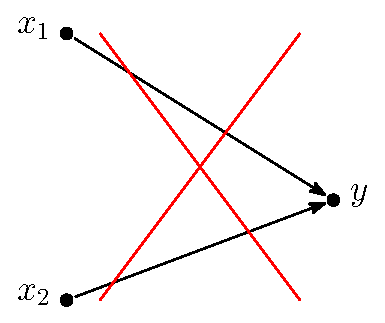
\includegraphics[width=0.25\textwidth]{4_1.eps}
	\caption{Не инъекция}
	\label{4_1}
\end{figure}

\textbf{Пример}: $x \mapsto x^2$ - не инъекция для всех чисел из $\mathbb{R}$, тогда как $x \mapsto x^3$ - инъекция

\begin{defn}
функция $f\colon X \rightarrow Y$ называется \uwave{сюръекцией}, если область значений функции $f$ совпадает с $Y$, то есть $\forall y \in Y, \exists\; x\in X \colon y = f(x)$. 
\end{defn} 


$x \mapsto x^2$, $X = \mathbb{R}$, $Y = \mathbb{R}$  - не сюръекция так как нет отрицательной части;\\
$x \mapsto x^2$, $X = \mathbb{R}$, $Y = \mathbb{R_+}$ - сюръекция;

\begin{figure}[H]
	\centering
	\begin{subfigure}[b]{0.5\textwidth}
		\centering
		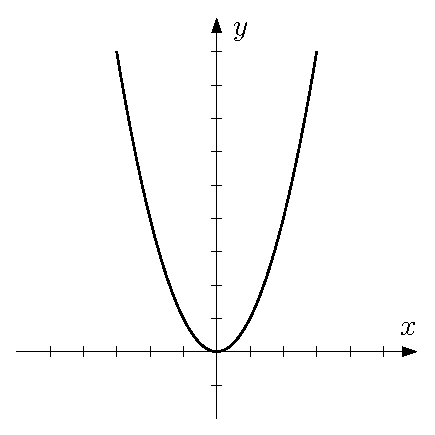
\includegraphics[width=4cm, height = 4cm]{4_2.eps}
		\caption{Не сюръекция}
		\label{4_2}
	\end{subfigure}
	\begin{subfigure}[b]{0.49\textwidth}
		\centering
		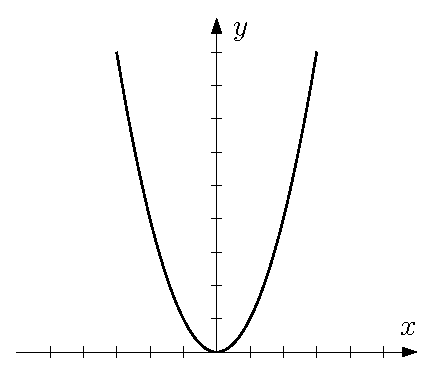
\includegraphics[width=4cm, height = 4cm]{4_3.eps}
		\caption{Сюръекция}
		\label{4_3}
	\end{subfigure}

	\caption{Примеры сюръективности}
	\label{fig:Сюръективность}
\end{figure}

\begin{defn}
Функция $f\colon X \rightarrow Y$ называется \uwave{биекцией}, если $f$ - инъекция и сюръекция одновременно, еще говорят - \uwave{взаимно-однозначное соответствие}.
\end{defn}
\begin{defn}
Если $\exists$ биекция $X\rightarrow Y$, то говорят, что $X$ и $Y$ - \uwave{равномощны}.
\end{defn}

\begin{prop} композиция биекций является биекцией:\\
$f\colon X \xrightarrow{\text{1-1}} Y,\, g\colon Y \xrightarrow{\text{1-1}} Z \Rightarrow g\circ f\colon X \xrightarrow{\text{1-1}} Z$
\end{prop}
\begin{proof}
$\forall x_1 \neq x_2,\, x_1, x_2 \in X \Rightarrow f(x_1) \neq f(x_2) \Longleftrightarrow y_1 = f(x_1) \neq f(x_2) = y_2 \Rightarrow g(y_1) \neq g(y_2) $\\ 
$\Rightarrow g\circ f$ - инъективна.\\
Так как $f$ - биъективна, то весь $Y$ - покрывается. Всеми элементами $Y$ покрывается множество $Z$, так как $g$ - биекция $\Rightarrow g\circ f$ - сюръекция.
\end{proof}

\begin{prop} \textbf{(существование)}
Если $f \colon X \rightarrow Y$ - биекция, то определяется функция из $Y$ в $X$, сопостовляющая $\forall y \in Y$ такой элемент $x \in X\colon y = f(x)$, эта функция называется обратной к $f$, обозначается $f^{-1}$ и является биекцией.
\end{prop}
\begin{proof}
Поскольку $f$ - сюръекция, то $\forall y \in Y, \, \exists x \in X$, так как f - инъекция, то $\forall y \in Y, \, \exists! x \in X \Rightarrow$ указанное сопостовление является функцией.\\
$f^{-1}$ - сюръекция, так как $\forall x \in X$ функция $f$ сопостовляет $y \in Y$, то есть: $\forall x \in X, \, \exists y \in Y \colon x = f^{-1}(y)$
$f^{-1}$ - инъекция, так как $\forall x \in X$ функция $f$ сопостовляет ровно один $y \in Y$, то есть: \\
$\forall y_1, y_2 \in Y \colon  y_1 \neq y_2,\, \exists x_1, x_2 \in X\colon x_1 = f^{-1}(y_1) \neq  f^{-1}(y_2) = x_2$. 
\end{proof}
 
\begin{figure}[H]
	\centering
	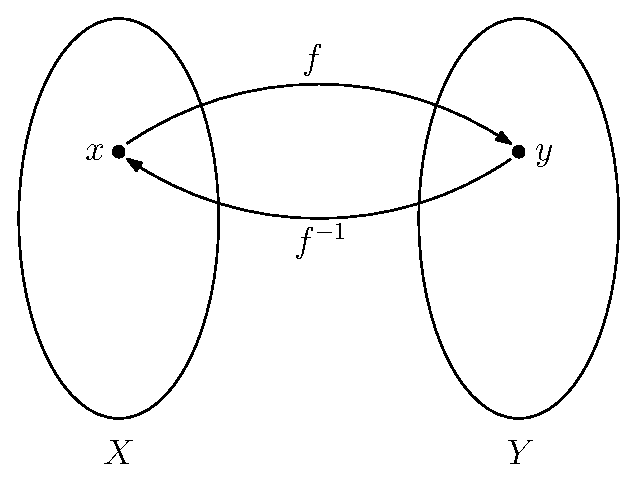
\includegraphics[width=0.3\textwidth]{4_4.eps}
	\caption{Обратная функция}
	\label{4_4}
\end{figure}

$x \rightarrow y \colon y^2 = x$ - это не функция.

Взаимосвязь между функцией и обратной функцией:
\begin{enumerate}
	\item $f^{-1}$ существует так как $f$ - биекция;
	\item $f^{-1}$ инъективна так как $f$ - функция;
	\item $f^{-1}$ сюръективна по определению $f$ как функции;
\end{enumerate}

\subsection*{Построение обратной функции}

Рассмотрим функцию $y = x^2$ - у неё нет обратной функции, так как это не биекция. Одному $y$ сопостовляется несколько $x$.
\begin{figure}[H]
	\centering
	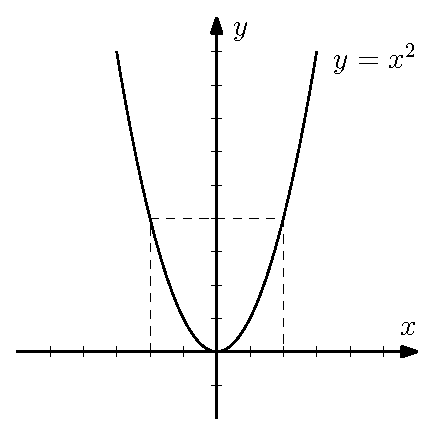
\includegraphics[width=0.3\textwidth]{4_5.eps}
	\caption{Функция без обратной функции}
	\label{4_5}
\end{figure}
Как сделать так, чтобы была обратная функция? Можно договорится какой $x$ берем для каждого $y$, например так:
\begin{figure}[H]
	\centering
	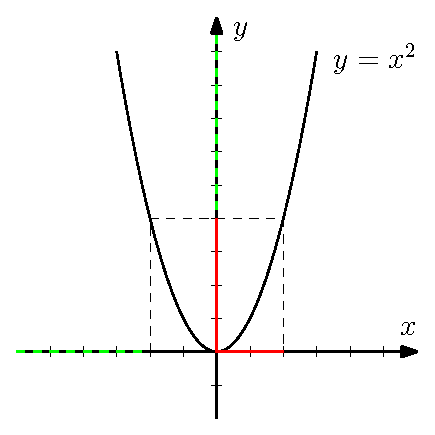
\includegraphics[width=0.3\textwidth]{4_6.eps}
	\caption{Способ выбора обратной функции}
	\label{4_6}
\end{figure}
С точки зрения сопоставления $y \rightarrow x \colon x^2 = y$ - все хорошо.\\
Рассмотрим немного другую функцию $y = x^2 \colon \{ x \geq 0 \} \rightarrow \{ y \geq 0 \}$.

\begin{figure}[H]
	\centering
	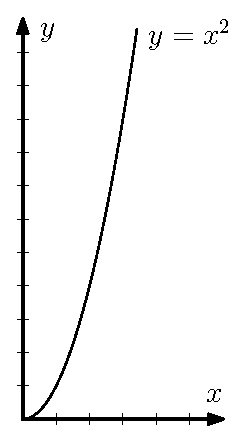
\includegraphics[width=0.15\textwidth]{4_7.eps}
	\caption{Функция с обратной функцией}
	\label{4_7}
\end{figure}
У этой функции есть биекция $\Rightarrow$ по утверждению существует обратная функция $x = \sqrt{y}$ - обратная функция. Непонятно, сюръекция ли эта функция или нет? Очевидно, что это инъекция.\\
Аналогично предыдущему примеру появился $\arcsin(.)$;

\textbf{Построение обратной функции}: либо функция сразу биекция, либо берется участок, где функция - биекция, а также должна проходится вся область значений, после этого строится обратная функция.

\newpage
\section*{Группы}

Пусть $X \neq \varnothing$, $G(X) = \{\, \text{все биекции } f\colon X \rightarrow X \,\}$ на $G(X)$ определена операция композиции $f\circ g$ - биекция, такая что:
\begin{enumerate}[label={(\arabic*)}]
	\item $f \circ ( g \circ h) = (f \circ g) \circ h$;
	\item $e(x) = x, \, e \circ f = f \circ e = f$;
	\item $\forall f, \, \exists f^{-1} \colon f^{-1} \circ f = f \circ f^{-1} = e$;
\end{enumerate}
тогда говорят, что задана \uline{группа биекций}.

\begin{defn}
Если на множестве задана бинарная операция, удовлетворяющая условиям (1)-(3), то говорят, что задана \uwave{группа}.
\end{defn}

\subsection*{Пример}
Возьмем $(\mathbb{Q}\setminus \{ 0 \}, \cdot)$, знаем что:
\begin{enumerate}
	\item $ (a \cdot b) \cdot c = a \cdot (b \cdot c), \, \forall a,b,c \in \mathbb{Q}$;
	\item $\exists 1 \colon 1 \cdot a = a \cdot 1 = a, \, \forall a \in \mathbb{Q}$;
	\item $\forall a \in \mathbb{Q}, \, \exists! a^{-1} \colon a^{-1} \cdot a = a \cdot a^{-1} = 1$;
\end{enumerate}
следовательно это группа по умножению. 

\uline{Группа биекций} - это универсальная группа, то есть любую группу можно представить как группу биекций (Теорема Кэли). Также существует дополнительно \uline{свойство коммутативности}:
\begin{enumerate}
\setcounter{enumi}{3}
	\item $ a \cdot b = b \cdot a$;
\end{enumerate}
Оно не выполняется для группы биекций.
\begin{exrc}
	Доказать, что $G(X)$ - коммутативна $\Leftrightarrow$ в $X$ - не более 2-х элементов. (В общем случае $G(X)$ не является абелевой группой).
\end{exrc}

\section*{Мощность множества}

См. выше определение.

\begin{prop}
Пусть $\{ a,b \} \subset A$ тогда $A\setminus \{ a \}$ равномощно  $A\setminus \{ b \}$.
\end{prop}

\begin{proof}
Пусть $D = A\setminus \{ a,b \} \Rightarrow A\setminus \{ a \} = D  \cup \{ b \},\, A\setminus \{ b \} = D  \cup \{ a \}, \, f \colon  A\setminus \{ a \} = D  \cup \{ b \} \rightarrow A\setminus \{ b \} = D  \cup \{ a \}$
	
Рассмотрим следующую функцию
\[ f(x) = \begin{cases} 
	x, & x \in D \\
	a, & x = b 
\end{cases}
\]
Легко заметить, что это наша искомая биекция. Проверим это: $y \in D \vee y = a \Rightarrow$ вся область значения покрывается $\Rightarrow$ функция - сюръекция.
$x_1 \neq x_2 \Rightarrow f(x_1) = x_1  \neq x_2 = f(x_2), \, \forall x_i \in D$. $x \neq a \Rightarrow f(x) = x \neq a = f(b), \, \forall x \in D \Rightarrow$ получаем инъекцию $\Rightarrow$ заданная функция является биекцией.
\end{proof}

\newpage

\subsection*{Свойства равномощных множеств}

Обозначение $A$ равномощно $B$ $\Leftrightarrow A \sim B$. Свойства равномощных множеств:
\begin{enumerate}[label={(\arabic*)}]
\item $A \sim A$ (тождественная биекция);
\item $A \sim B \Rightarrow B \sim A$ (так как обратная функция - биекция);
\item $A \sim B \wedge B \sim C \Rightarrow A \sim C$ (так как композиция биекций - биекция);
\end{enumerate}
Обычно ``мощность'' не употребляют в контексте просто множества, так как это ведет к понятию множества всех множеств. Употребляют обычно ``равномощно'', поскольку мощность можно интерпретировать как класс эквивалентности ``среди всех множест'' - что не есть хорошо (получается множество все множеств).\\

\begin{prop}
$\{\, k \in \mathbb{N}\mid k \leq n \,\} \sim \{\, k \in \mathbb{N}\mid k \leq m \,\}$, то $n = m$.
\end{prop}

Интуитивно хочется поставить стрелочки и потом сказать ``и так далее'' - плохое объяснение.
 \begin{figure}[H]
	\centering
	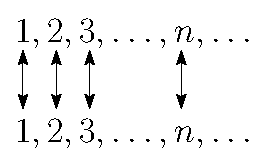
\includegraphics[width=0.2\textwidth]{4_8.eps}
	\caption{Сопоставление множеств}
	\label{4_8}
\end{figure}

\begin{proof}
Индукцией по $n$:\\
\uline{База}: $n =1 \Rightarrow$ пусть $m \neq 1$, $f$ - биекция $f \colon \{\, k \leq n \,\} \rightarrow \{\, k \leq m \,\}$.
Так как $n = 1$, то $\{ k \leq n \} = \{ 1 \}$. Тогда $f(1) \neq m \vee f(1) \neq 1$, иначе они между собой равнялись бы ($m=1$) $\Rightarrow f$ - не сюръекция, так как область значений состоит из $f(1)$ которая не равна $m$ или 1 $\Rightarrow$ не все элементы в образе - заметаются, то есть в $\{\, k \in \mathbb{N}| k \leq m \,\}$ будут элементы меньше $m \Rightarrow$ противоречие с тем, что $f$ - биекция $\Rightarrow m = 1$.\\
\uline{Шаг}: Пусть доказано для $n$, докажем для $n+1$. Есть биекция $\{1,2,...,n,n+1\} \xrightarrow{f} \{1,2,...,m\}$.\\
Если $m = 1$, то все доказано (см. базу): в этом случае возьмем обратную функцию, обратная функция - биекция и по утверждению из базы будет следовать, что $n + 1 = 1$, но такое невозможно, так как 1 не является ни для кого следующей, поэтому $m \neq 1$ по утверждению в базе.\\
$\{1,2,\dotsc,n\} \xrightarrow{f} \{1,2,\dotsc,m\} \setminus \{f(n+1)\}$ - убираем образ $n+1$.
 
 \begin{figure}[H]
 	\centering
 	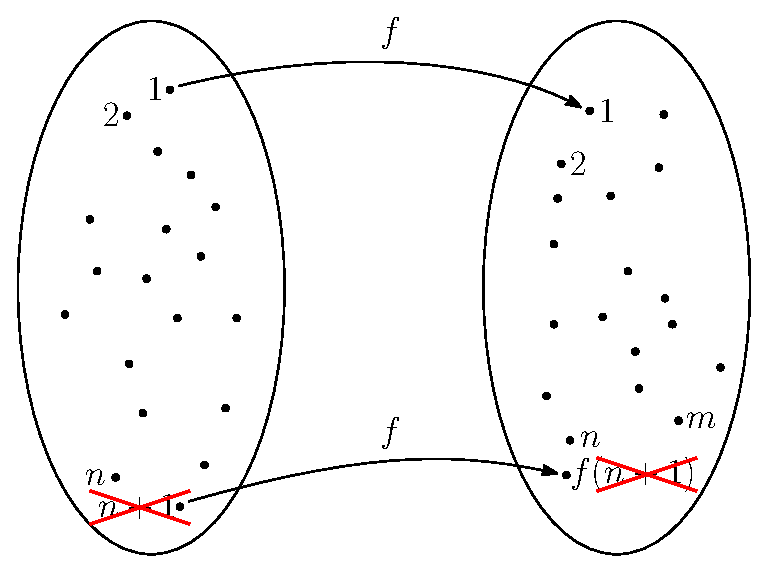
\includegraphics[width=0.4\textwidth]{4_9.eps}
 	\caption{Убираем образ $n+1$}
 	\label{4_9}
 \end{figure}
Не важно, что выбрасывать с точки зрения равномощности:\\ 
$ \{1,2,\dotsc,n\} \xrightarrow{f} \{1,2,\dotsc,m\} \setminus \{f(n+1)\} \sim \{1,2,\dotsc,m-1\}$ 
 по утверждению выше. Таким образом получим: $\{1,2,\dotsc, n\} \sim \{1,2,\dotsc, m-1\} \Rightarrow$ по предположению индукции получим, что $n = m-1$, добавляем единичку, получаем $n + 1 = m$ 
\end{proof} 

\begin{defn}
	Пустое множество $\varnothing$ - является \uwave{конечным} и состоит из \uline{0 элементов}. Множество $A$ является \uwave{конечным} и состоит из \uline{$n$ элементов}, если $A \sim \{1,2,...,n\}$. 
\end{defn}

\begin{defn}
	\uwave{Бесконечное множество} - множество, которое не является конечным множеством.
\end{defn}

\begin{rem}
	Конечныe множества - те, которые можно посчитать.
\end{rem}


\subsection*{Примеры бесконечных множеств}
\begin{prop}
	Множество натруальных чисел $\mathbb{N}$ - бесконечно (не является конечным). 
\end{prop}
\begin{proof}
(От противного): Пусть $\mathbb{N}$ - конечно $\Rightarrow \exists f$ - биекция $f \colon \{1,2,\dotsc,m\} \rightarrow \mathbb{N}$.\\
Возьмем натуральное число $f(1)+\dotsc+f(m)+1> f(k), \, \forall k = 1,\dotsc,m \Rightarrow f$ - не сюръекция.
Значит множество натуральных чисел - бесконечно.
\end{proof}

\begin{prop}
	Множество простых чисел - бесконечно.
\end{prop}

\begin{proof}
Пусть есть биекция $f \colon \{1,\dotsc,m\}\rightarrow \text{prime}$. Пусть $p_1, p_2, ..., p_m$ - все простые числа.\\ 
Составляем новое $p_1p_2\dotsc p_m +1$ - больше любого из выписанных $\Rightarrow$ это составное число $\Rightarrow$ делится на какое-то простое, но это невозможно, так как оно не может делится ни на одно простое число $\Rightarrow$ противоречие.
\end{proof}

\begin{defn}
	Множество $A$ - \uwave{счетно}, если $A \sim \mathbb{N}$. То есть элементы множества можно пересчитать.
\end{defn}

\subsection*{Примеры счетных множеств}
\begin{enumerate}
	\item $\mathbb{N}$, биекция: $n \rightarrow n$;
	\item $\mathbb{N}\setminus \{1\}$, биекция: $n \rightarrow n+1$;
	\item $\mathbb{Z}$, данное множество состоит из $\{\,-n \mid n \in \mathbb{N} \,\},\, \{0\},\, \mathbb{N}$.\\ Сопоставление: $0,1,-1,2,-2,3,-3, \dotsc \Leftrightarrow 1\rightarrow 0, 2 \rightarrow 1, 3 \rightarrow -2, \dotsc$;
\end{enumerate}

\subsection*{Свойства счетных множеств}

(1) Если $A$ счетно и $B \subset A$, то $B$ - конечно или счетно $\Leftrightarrow$ не более, чем счетно (н.б.ч.с.).
\begin{proof}
	Все элементы $A$ - пересчитаны: $\{a_1, a_2, a_3, \dotsc\}$.
	
	Если $B = \varnothing$ - все ок, так как пустое множество является конечным и состоит из 0 элементов.
	
	Пусть  $B \neq \varnothing$, положим, что $k_1 = \min\{\, k\colon a_k \in B\,\}$. Такое существует, так как в любом непустом подмножестве натуральных чисел есть наименьший элемент (аксиома индукции). Пусть $b_1 = a_{k_1} \Rightarrow$ если $B \setminus \{b_1\} = \varnothing$, то $B$ - конечно $\Rightarrow$ ok.\\ 
	Если $B \setminus \{b_1\} \neq \varnothing$, то берем $k_2 = \min\big\{\,k\colon a_k \in B \setminus \{b_1\}\,\big\}$ и полагаем $b_2 = a_{k_2}$ и далее по аналогии.
	
	Если уже построили $\{b_1, \dotsc , b_n\}$, то либо $B \setminus \{b_1, \dotsc, b_n\} = \varnothing$ и тогда построение закончено, или\\ 
	$B \setminus \{b_1, \dotsc , b_n\} \neq \varnothing$ и определяем $k_{n+1} = \min\big\{k\colon a_k \in B \setminus \{b_1, \dotsc , b_n\}\big\}$, полагая $b_{n+1} = a_{k_{n+1}}$ продолжаем по аналогии. Получаем набор $\{b_n\}$. Верно ли что $B = \{b_n\}$? (все ли элементы так прошли?)
	
	Покажем, что $k_n \geq n$: \\
	$k_1 \geq 1$ - очевидно, так как берем натуральные числа. $k_{n+1} > k_n$ - так как берем каждый раз минимальный номер. По индукции, $k_n \geq n \Rightarrow k_{n+1} \geq n+1$ поскольку $k_{n+1} > k_n \geq n$ - строго больше $n$, то есть больше или равно $n+1$.
	
	Если процедура закончилась, то по построению $B$ - полностью перенумерован.
	
	Предположим, что построение не прерывалось на конечном шаге (продолжалось бесконечно долго) и какой-то $a_m \in B$ не получил номера. Но так как мы выбирали каждый раз наименьшие номера $\Rightarrow k_n < m, \, \forall n$, но $k_{m+1} \geq m + 1$ (Если какое-то число просмотрели $\Rightarrow$ все выбираемые номера - меньше него, но меньше него есть только конечный набор чисел, а построение никогда не обрывалось $\Leftrightarrow$ бесконечный набор чисел.) $\Rightarrow$ противоречие.
\end{proof}

\end{document}